\chapter[Revisão de Literatura]{Revisão de Literatura}

%\addcontentsline{toc}{chapter}{Revisão de Literatura}
% ----------------------------------------------------------

Nesse capítulo é feita uma revisão no estado da arte dos algoritmos de roteamento de veículos a aplicação de algoritmos genéticos para mesma finalidade.

\section{Roteamento de Veículos com Janelas de Tempo}

Um dos problemas mais importantes de otimização combinatória e mais estudados na literatura de pesquisa operacional é o problema de Roteamento de Veículos com Janelas de Tempo (PRVJT).
Nele consiste que tendo uma frota de veículos que deve partir de um depósito, deve atender a demanda de N consumidores e retornar ao depósito de forma que o custo total de viagem seja o mínimo. Levando em consideração que o atendimento aconteça dentro de um intervalo de tempo especificado para cada consumidor. Também deve-se respeitar a capacidade dos veículos.

Na literatura existem vários objetivos abordados pelos autores para o PRVJT.\ Neste trabalho temos como objetivo a minimização da distancia total percorrida, que é o mais comum na literatura.~\cite{ROCHAT}

\subsection{Formulação matemática}

O PRVJT pode ser definido a partir um grafo completo orientado~\(G = (V,A)\) em que \(V = {0,\cdots,n+1}\) é um conjunto de vértices e \(G ={(i,j)|i,j \in V}\) é o conjunto de arcos.
Cada arco (i,j) é associado a um tempo \(t_{ij}\) e um custo de travessia \(c_{ij}\).

É necessário uma definição precisa do termo \textit{custo de travessia}. Em casos práticos pode se considerar diversos fatores, tais como distancia, tempo, desgaste do veículo ao percorrer determinado caminho, entre outros fatores. Porém, quando se trata de problemas teóricos envolvendo janelas de tempo, é comum converter todas as medidas relevantes em unidades de tempo para fins de padronização e também para facilitar a comparação entre diferentes métodos. Por isso, adota-se aqui a mesma definição de custo que a maioria dos trabalhos teóricos da literatura, considerando que o custo de viagem consiste na distância convertida em unidades de tempo.

Podemos descrever o problema como sendo um conjunto \(K\) de veículos com capacidade \(Q\), eles devem atender \(n\) clientes, representados pelos vértices \(1,\cdots,n\). Considera-se que \(N = V \{0, n + 1\}\) representa o conjunto de clientes. Os veículos devem partir do depósito e, após visitar todos os clientes, devem retornar ao mesmo local de onde partiram. Por conveniência, o deposito é representado por dois vértices, o vértice \(0\), que representa a origem, e o vértice \(n+1\) que representa o destino. A cada cliente \(i\), uma demanda \(q_i\) é associada, esta deve ser atendida por um único veículo. E todos os vértices possuem uma janela de tempo \([e_i,l_i]\), o serviço no vértice \(i\) deve ser iniciado dentro desse intervalo. Caso ocorra que a chegada ao cliente \(i\) aconteça antes do horário previsto \(e_i\), ele deve esperar a abertura da janela. O veículo não poderá chegar a \(i\) depois do instante \(l_i\), pois isso faria violar a restrição de tempo do problema. Esse tipo de restrição é conhecido na literatura como janela de tempo rígida. A cada vértice é também associado um tempo de serviço, denotado por \(s_i\). O objetivo é encontrar uma solução \(s\) de custo mínimo, de forma a minimizar a soma de todos os custos de viagem \(\sum_{(i,j) \in s} c_{ij}\) que são associados aos arcos \((i,j)\) presentes nas rotas que compõem essa solução.

A formulação matemática do PRVJT, é apresentada pelas expressões:

\begin{equation}  \label{eq:prvjt1}
\min
 \sum_{k \in K}\sum_{i \in V}\sum_{j \in V} c_{ij}x_{ijk}
\end{equation}

Sujeito as seguintes restrições:

\begin{equation} \label{eq:prvjt2}
\sum_{k \in K}\sum_{j \in V} x_{ijk} = 1, \forall i \in N
\end{equation}

\begin{equation} \label{eq:prvjt3}
\sum_{j \in V} x_{0jk} = 1, \forall k \in K
\end{equation}

\begin{equation} \label{eq:prvjt4}
\sum_{i \in V} x_{ijk} - \sum_{i \in V} x_{jik} = 0, \forall k \in K, \forall j \in N
\end{equation}

\begin{equation} \label{eq:prvjt5}
\sum_{i \in V} x_{i(n+1)k} = 1, \forall k \in K
\end{equation}

\begin{equation} \label{eq:prvjt6}
\sum_{i \in N} q_i \sum_{j \in V} x_{ijk} \leq Q, \forall k \in K
\end{equation}

\begin{equation} \label{eq:prvjt7}
b_{ik} + s_i + t_{ij} -(1-x_{ijk})M_{ij} \leq b_{jk},\forall k \in K, \forall (i,j) \in A
\end{equation}

\begin{equation} \label{eq:prvjt8}
e_i \leq b_{ik} \leq l_i,\forall k \in K,\forall i \in V
\end{equation}

\begin{equation} \label{eq:prvjt9}
x_{ijk} \in \{0,1\},\forall k \in K,\forall (i,j) \in A
\end{equation}

A variável binária \(x_{ijk}\) assume valor 1 se o veículo \(k\) passa pelo arco (i,j) e 0, caso contrário.

A função objetivo \ref{eq:prvjt1} expressa o custo total a ser minimizado. 
As restrições \ref{eq:prvjt2} asseguram que somente um veículo \(k\) parte de cada cliente \(i\). 
As restrições \ref{eq:prvjt3}, \ref{eq:prvjt4}, \ref{eq:prvjt5} garantem a continuidade do caminho a ser percorrido pelo veículo \(k\), ou seja, cada veículo parte do depósito, visita os clientes e em seguida retorna ao depósito. 
As restrições \ref{eq:prvjt6} fazem com que cada veículo \(k\) somente possa atender a um conjunto de clientes cuja demanda total não ultrapasse sua capacidade Q. 
As restrições \ref{eq:prvjt7}, \ref{eq:prvjt8} asseguram a viabilidade das rotas no que diz respeito as restrições de janelas de tempo, em que \(b_{ik}\) representa o tempo em que o veículo \(k\) começa a atender o cliente \(i\) e \(M_{ij}\) são constantes de valor suficientemente grande.  As restrições \ref{eq:prvjt9} definem o domínio das variáveis de decisão.~\cite{CORDEAU}


\subsection{Complexidade}

Encontrar a solução ótima do PRVJT implica em obter simultaneamente a solução de vários problemas NP-difíceis, dentre os quais citam-se o \textit{Problema do Caixeiro Viajante} (PCV) e o \textit{Problema da Mochila}. Sendo assim, tal tarefa é também NP-difícil. Além disso, encontrar uma simples solução viável para o PRVJT dispondo de um conjunto limitado de veículos é NP-difícil no sentido forte \cite{Kohl}. Porém, uma solução inicial viável é trivial caso o número de veículos seja ilimitado, bastando atender cada consumidor com um veículo.

Os atuais resultados encontrados na literatura referentes ao PRVJT comprovam que os algoritmos exatos restringem-se à resolução de problemas-teste com tamanho reduzido e janelas de tempo apertadas. Embora hoje podemos resolver problemas com um tamanho que seja ligeiramente maior que o de alguns anos atrás, o crescimento da capacidade dos computadores e da eficiência dos algoritmos esta muito distante da curva exponencial representada por este problema. Pode-se dizer que os métodos exatos não são uma alternativa viável para situações onde a um número maior de consumidores, como ocorre na maioria dos casos reais. \cite{Chabrier}

Abordagens heurísticas e algoritmos aproximativos também tem sido utilizadas na resolução do PRVJT. As Heurísticas buscam obter uma solução em tempo hábil. Este fato torna as estratégias heurísticas muito poderosas se comparadas com abordagens exatas, que focam exclusivamente na obtenção da solução ótima. Uma boa heurística deve ser capaz de encontrar soluções próximas da ótima, em tempo bem inferior ao necessário pelos métodos exatos. A qualidade da solução não deve variar demasiadamente ao aplicá-la em diferentes ou ao mesmo problemas-teste. Até 2006, 45 do total de 56 problemas de Solomon tiveram uma solução ótima. Alguns casos foram gastos mais que cinco horas de processamento na resolução de algumas instancias, enquanto em outras puderam ser resolvidas em menos de um minuto. ~\cite{Jepsen}

Os métodos aproximativos vem ao encontro destas características. Um método aproximativo é uma heurística com garantia de qualidade no resultado. A melhor solução encontrada por um algoritmo de aproximação esta sempre a uma distancia percentual previamente definida da solução ótima desconhecida. A "distancia do ótimo" é particular de cada algoritmo, podendo até não ser muito relevante em termos práticos. Um exemplo bem conhecido é o algoritmo PRIM, para árvore geradora mínima, que é capaz de oferecer uma solução viável para o PCV, que é no máximo duas vezes o ótimo em distancia total percorrida \cite{Alvarenga}.

Dado essa complexidade, resolver esse problema utilizando de abordagens puramente exatas é uma tarefa extremamente árdua, demandando tempo computacional muito elevado. Por isso é motivado o desenvolvimento de novos algoritmos heurísticos com tempos mais reduzidos para a solução do PRVJT, mesmo que esses não garantam uma solução ótima.

\subsection{Heurísticas}

Heurísticas são procedimentos de busca que visam a obtenção de soluções com uma qualidade satisfatória em um tempo computacional aceitável. Porem tais procedimentos não garantem encontrar a solução ótima nem são capazes de mensurar o quão próxima a solução obtida está da ótima. Sera enumerado as ideias centrais de algumas heurísticas construtivas e de refinamento disponíveis na literatura.

\subsubsection{Construção de rotas}

Um dos trabalhos mais antigos sobre heurística para construção de rotas para PRVJT proposto por Baker \cite{Baker} em 1989, Foi criada a partir da ideia da heurística das economias de Clarke e Write \cite{Clarke} que foi proposta para criação de soluções para o PRV. O algoritmo funciona primeiramente criando uma rota partindo do depósito para cada cliente \textit{i}, para em seguida varias iterações ocorrerem, para cada o algoritmo calcula quais duas rotas que podem ser combinadas de forma a gerar a maior economia possível.

Outra heurística proposta por \cite{VANLANDEGHEM} também baseada na heurística das economias é uma heurística de dois critérios, nesta as janelas de tempo são utilizadas para mensurar o quanto uma ligação entre dois clientes é boa em termos de tempo.

De forma semelhante \cite{Solomon} desenvolveu um algoritmo baseado na ideia na heurística das economias para resolução do PRVJT. Devido a existência de janelas de tempo, deve-se considerar também a orientação da tora. Também deve-se checar as violações de janelas de tempo quando mais de uma rota é combinada. Ela de forma igual a heurística das Economias original possuem complexidade \(O^2 log n^2\).
Nesta heurística toda rota é inicializada encontrando o cliente mais próximo ao depósito que ainda não pertença a nenhuma rota. A cada iteração subsequente o cliente mais próximo ao último adicionado à rota é considerado para inserção ao final da rota que está sendo gerado. Quando a busca falha, uma nova rota é inicializada.



\subsubsection{Aprimoramento de rotas}
\subsubsection{Estruturas de vizinhança}

\subsection{Metaheurísticas}

% https://en.wikibooks.org/wiki/LaTeX/Mathematics
\section{Algoritmos genéticos}

AG é uma técnica amplamente utilizada de IA, que utilizam conceitos provenientes do princípio de seleção natural para abordar uma  ampla série de problemas, geralmente de adaptação. \cite{DiogoCLucas}

\subsection{Funcionamento}
 
Inspirado na maneira como o seleção natural explica o processo de evolução das espécies, Holland \cite{Holland1975} decompôs o funcionamento dos AG em sete etapas, essa são \textit{inicialização}, \textit{avaliação}, \textit{seleção}, \textit{cruzamento}, \textit{mutação}, \textit{atualização} e  \textit{finalização} conforme a Figura \ref{fig:EstruturaAG}. 

\begin{minipage}{\linewidth}
    \makebox[\linewidth]{
        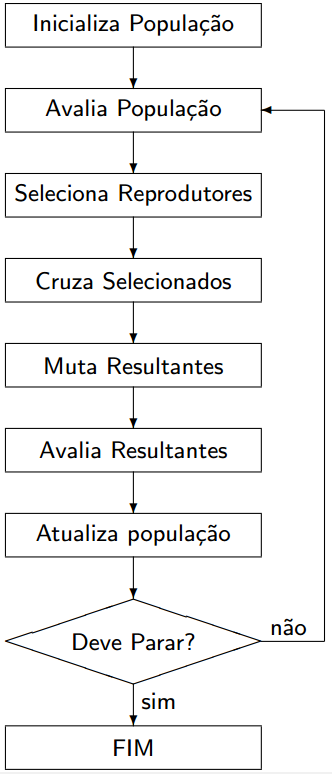
\includegraphics[keepaspectratio=true,scale=0.45]{ibagens/genetico1.png}}
    \captionof{figure}{Estrutura de um AG \cite{DiogoCLucas} }
    \label{fig:EstruturaAG}
\end{minipage}


\subsection{Inicialização}
Criar uma população de possíveis respostas para um problema. 
É comum fazer uso de funções aleatórias para gerar os indivíduos, sendo este um recurso simples que visa fornecer maior diversidade.

\subsection{Avaliação}
Avalia-se a aptidão das soluções, os indivíduos da população, então é feita uma análise para que se estabeleça quão bem elas respondem ao problema proposto.
A função de avaliação também pode ser chamada de função objetivo. Ela pode variar de acordo com problema,  
Calcular com exatidão completa o grau de adaptação dos indivíduos pode ser uma tarefa complexa em muitos casos, e se levarmos em conta que esta operação é repetida varias vezes ao longo do processo de evolução, seu custo pode ser consideravelmente alto. Em tais situações é comum o uso de funções não determinísticas, que não avaliam a totalidade das características do indivíduo, operando apenas sobre uma amostragem destas.

\subsection{Seleção}
Ela é a responsável pela perpetuação de boas características na espécie. 
Neste estágio que os indivíduos são escolhidos para posterior cruzamento, fazendo uso do grau de adaptação de cada um é realizado um sorteio, onde os indivíduos com maior grau de adaptação tem maior probabilidade de se reproduzirem.
O grau adaptação é calculado a partir da função de avaliação para cada individuo, determina o quão apto ele esta para reprodução relativo a sua população. 

\textbf{Selection Random}: Gera um numero aleatório entre 0 e o tamanho total da população e retorna o indivíduo do índice escolhido.

\textbf{Selection Roulette Wheel}: Faz a soma de todos os valores da função de aptidão da população, depois calcula a porcentagem de cada indivíduo referente ao total 
e guarda em um vetor. Então é gerado um valor A aleatório entre 0 e 1 e multiplicado pelo valor total dos pesos. Para selecionar o indivíduo é feito um loop 
nos pesos e seus valores somados até que o valor A seja igual ou menor que zero, o índice do peso que fez a condição acontecer, se o índice do indivíduo selecionado.
Desta forma aumentando a possibilidade de selecionar um indivíduo com maior aptidão.

\subsection{Cruzamento}
Características das soluções escolhidas na seleção são recombinadas, gerando novos indivíduos.

\textbf{CrossOver Simple}: Utiliza dois indivíduos selecionados,  define dois números aleatórios de 0 até menor tamanho da lista de cromossomos entre os dois, 
sendo que o primeiro índice tem que ser menor que o segundo índice e os mesmos não podem ser iguais. 
Esse tamanho é utilizado para trocar cromossomos entre os dois indivíduos, ou seja, adicionar todos os cromossomos do primeiro indivíduo do índice 
igual ao primeiro numero, até o índice segundo numeSAro, e repete o processo contrario.

\textbf{Crossover OBX (Order-Based Crossover)}: Utiliza dois indivíduos escolhidos na seleção, então define dois números aleatórios, de 0 até menor tamanho da lista de cromossomos entre os dois, sendo que o primeiro tem que ser menor que o segundo e não podem ser iguais. O primeiro numero até o segundo numero, são definidas posições aleatórias e são salvas em uma lista. Faz um loop na lista e troca o cromossomo da posição do primeiro indivíduo para o segundo e do segundo para o primeiro.

\textbf{Crossover PBX (Position-Based Crossover)}: Utiliza dois indivíduos selecionados, então define dois números aleatórios, 
de 0 até menor tamanho da lista de cromossomos entre os dois, sendo que o primeiro índice tem que ser menor que o segundo índice e os mesmos não podem ser iguais. 
Entre esse tamanho são definidas posições aleatórias e guardadas em uma lista. Os indivíduos resultantes são zerados, 
e para cada posição é trocado do cromossomo principal para o resultante de mesma posição outro da mesma posição. 
As posições não preenchidas são completadas com os cromossomos restante, seguindo a ordem do cromossomo e adicionado se ele não ja existir na lista.

\subsection{Mutação}
Características dos indivíduos resultantes do processo de reprodução são alteradas, acrescentando assim variedade a população.
A mutação opera sobre os indivíduos resultantes do processo de cruzamento e com uma probabilidade pré-determinada efetua algum tipo de alteração em sua  estrutura. A importância desta operação é o fato de que uma vez bem escolhido seu modo de atuar, é garantido que diversas alternativas serão exploradas.

\textbf{MutateEM (Exchange Mutation)}: Define duas das posições aleatórias distintas do segundo cromossomo até o ultimo, e troca os cromossomos do indivíduo.

\textbf{MutateSM (Scramble Mutation)}: Define duas das posições aleatórias distintas do segundo cromossomo até o ultimo, e uma quantidade aleatória. Então faz um loop da quantidade aleatória e mistura os cromossomos que estão entre a posição inicial e final trocando aleatoriamente dois pontos entre eles.

\textbf{MutateDM (Displacement Mutation)}: Define duas das posições aleatórias distintas do segundo cromossomo até o ultimo, e remove todos os cromossomo entre essa posições e recoloca a partir de uma posição aleatória.

\textbf{MutateIM (Insertion Mutation)}: Define uma posição aleatória, remove o cromossomo da posição, reorganiza os cromossomos e insere o cromossomo removido em uma nova posição aleatória.

\textbf{MutateIVM (Inversion Mutation)}: Define duas das posições aleatórias distintas do segundo cromossomo até o ultimo, e inverte todos os cromossomos que está entre as posições.

\textbf{MutateDIVM (Displaced Inversion Mutation)}:Define duas das posições aleatórias distintas do segundo cromossomo até o ultimo, e remove todos os cromossomo entre essa posições e recoloca a partir de uma posição aleatória de forma invertida.

\subsection{Atualização}
Os indivíduos criados no processo de reprodução e mutação são inseridos na população.

Na forma mais tradicional deste a população mantém um tamanho fixo e os indivíduos são criados em mesmo número que seus antecessores e os substituem por completo. 

Existem, porém, algumas alternativas, o número de indivíduos gerados pode ser menor ou o tamanho da população pode sofrer variações e o critério de inserção pode variar, por exemplo, nos casos em que os filhos substituem os pais, ou em que estes só são inseridos se possuírem maior aptidão que o cromossomo que sera substituído, ou o manter sempre o conjunto dos n melhores indivíduos. 

\subsection{Finalização}
É testado se as condições de encerramento da evolução foram atingidas, retornando para a etapa de avaliação em caso negativo e encerrando a execução em caso positivo.

Os critérios para a parada podem ser vários, desde o número de gerações criadas até o grau de convergência da população atual.


Toda base dos AG se fundamenta nos indivíduos, eles são a unidade básica em qual o algoritmo se baseia, sua função é codificar as possíveis soluções do problema a ser tratado e partir de sua manipulação no processo evolutivo, a partir daí que são encontradas as respostas.

Esses indivíduos precisam de uma representação, essa será o principal responsável pelo desempenho do programa. É comum chamar de \textit{genoma} ou \textit{cromossomo} para se referir ao individuo. Por essa definição podemos resumir um indivíduo pelos genes que possui, ou seja seu \textit{genótipo}.

Apesar de toda representação por parte do algoritmo ser baseada única e exclusivamente em seu genótipo, toda avaliação é baseada em seu fenótipo, o conjunto de características observáveis no objeto resultante do processo de decodificação dos genes do individuo, ver Tabela 1.

\newcolumntype{C}[1]{>{\centering\let\newline\\\arraybackslash\hspace{0pt}}m{#1}}
\begin{table}[h]
    \centering
\vspace{0.5cm}
\renewcommand{\arraystretch}{2.0}
\caption{Exemplos de genótipos e fenótipos correspondentes em alguns tipos de problemas \cite{DiogoCLucas}}
    \begin{tabular}{|C{4cm}|C{3.5cm}|C{7cm}|}
        \hline
        \textbf{Problema} & \textbf{Genótipo} & \textbf{ Fenótipo} \\
        \hline                  
        Otimização numérica & 0010101001110101 & 10869 \\
        \hline
        Caixeiro viajante & CGDEHABF & Comece pela cidade C, depois passe pelas cidades G, D, E, H, A, B e termine em F \\
        \hline
        Regras de aprendizado para agentes & C$_1$R$_4$C$_2$R$_6$C$_4$R$_1$ & Se condição 1 (C$_1$) execute regra 4 (R$_4$), se (C$_2$) execute (R$_6$), se (C$_4$) execute (R$_1$)\\
        \hline
    \end{tabular}
\end{table} 

Para cada indivíduo é calculado o seu grau de adaptação, a partir de uma função objetivo, comumente denotada como na formula \ref{eq:solve0}.

\begin{equation} \label{eq:solve0}
f_O(x)  
\end{equation}


Que vai representar o quão bem a resposta apresentada pelo individuo soluciona o problema proposto.

Também é calculado o grau de adaptação do indivíduo relativo aos outros membros da população a qual ele pertence, esse é chamado de grau de aptidão, para um indivíduo $x$ temos seu grau de aptidão denotado pela fórmula \ref{eq:solve1}.


\begin{equation} \label{eq:solve1}
    f_A(x) = \frac{f_O(x)}{ \sum_{i=1}^{n}  f_O(i)  }  
\end{equation}


 Sendo n o tamanho da população.
 
 A dinâmica populacional é a responsável pela evolução, ao propagar características desejáveis a gerações subsequentes no processo de cruzamento, enquanto novas são testadas no processo de mutação.
 
 Algumas definições importantes relativo as populações de um AG são:
 
 \textbf{Geração:} É o número de vezes em que a população passou pelo processo de seleção, reprodução, mutação e atualização.

\textbf{Média de adaptação:} É a taxa média que ao indivíduos se adaptaram ao problema, é definida pela formula \ref{eq:solve2}. 

\begin{equation} \label{eq:solve2}
M_A = \frac{ \sum_{i=1}^{n} f_O(i) }{n}
\end{equation}


\textbf{Grau de convergência:} define o qual próxima esta a media de adaptação desta população relativo as anteriores. O objetivo dos AG é fazer a população convergir para uma valor de adaptação ótimo.
Um estado negativo que pode ocorrer relativo a esta medida é a \textit{convergência prematura}, a mesma ocorre quando a população converge em uma média de adaptação sub-ótima, e dela não consegue sair por causa de sua baixa diversidade.

\textbf{Diversidade:} Mede o grau de variação entre os genótipos da população. Ela é fundamental para o tamanho da busca.
Sua queda esta fortemente ligada ao fenômeno de \textit{Convergência prematura}.

\textbf{Elite:} São os indivíduos mais bem adaptados da população. Uma técnica comum nos AG é p \textit{elitismo}, onde são selecionados k melhores indivíduos que serão mantidos a cada geração.

\subsection{Aplicações}
Existem vários aplicações para os algoritmo genéticos, por serem uma inteligência artificial não supervisionada, de rápido aprendizado e podendo ser paralelizado.

O modelo m-PRC(Problema de Rotas de Cobertura multi-veículo) é uma aplicação de algoritmos genéticos para construção de rotas em uma região mapeada, para encontrar uma boa distribuição de viaturas para patrulhamento urbano usado por departamentos de segurando como a policia, guardas municipais ou segurança privada \cite{Washington}. 
O Modelo é definido como um grafo não direcionado \ref{eq:solve3}. 

\begin{equation} \label{eq:solve3}
G=(V\cup W, E)
\end{equation}

Onde \ref{eq:solve4}: 

\begin{equation} \label{eq:solve4}
V\cup W
\end{equation}


Compõem o conjunto de vértices e E o conjunto de arestas, ou seja, o subgrafo induzido por E e um grafo completo cujo conjunto de nós é V. 
V são todos os vértices que podem ser visitados e é composto pelo subconjunto T, que são os vértices que devem ser visitados por algum veiculo. W é um conjunto de vértices onde todos os M veículos devem passar. M é o numero de rotas de veículos que começam no vértice base V$_0$. 

O m-PRC atribui o conjunto de m rotas de veículos com as restrições: todas as m rotas de veículos começam e terminam na base V$_0$, Tem exatamente m rotas, cada vértice de V pertence a no máximo uma rota, cada vértice de T pertence a exatamente uma rota, com exceção a base, cada vértice de W deve ter uma rota que passa por ele e em uma distancia C de um vértice V visitado, O modulo da diferença entre o número de vértices de diferentes rotas não pode exceder um determinado valor R. A Figura \ref{fig:GrafoVUW} mostra o grafo da relação de V com W.

\begin{minipage}{\linewidth}
    \makebox[\linewidth]{
        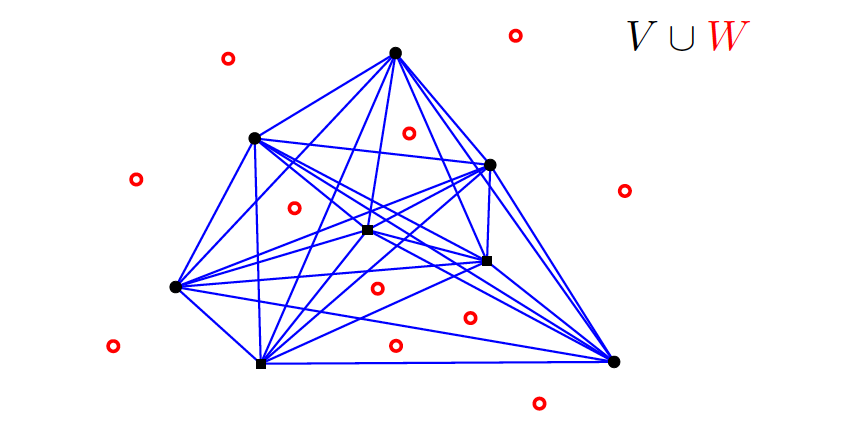
\includegraphics[keepaspectratio=true,scale=0.5]{ibagens/grafoMPRC.png}}
    \captionof{figure}{Exemplo de gráfo não direcionado para V U W. \cite{Washington} }
    \label{fig:GrafoVUW}
\end{minipage}

Para utilizar o algoritmos genéticos com o modelo m-PRC, o trabalho propõem dois modelos. O AGS (Algoritmo genético sequencial), que utiliza heurísticas GENIUS e 2-opt balanceada para ajustes finais para tentar melhor a solução; O AGH(Algoritmos genéticos H-1-PRC), que utiliza heurísticas H-1-PRC-MOD e 2-opt balanceada em todo o processo de resolução.

A conclusão de \cite{Washington} é que a utilização de algoritmos genéticos para a resolução de de uma adaptação do problema de rotas de cobertura de veículos como bastante relevantes e de fácil manipulação. O modelo AGS resolve o problema de forma rápida e tem uma fácil implementação dentro dos critérios de comparação adotadas. O modelo AGH é mais lento e não conseguiu encontrar a solução para alguns exemplos.


